\documentclass{beamer}
\usepackage{lmodern} % Allows arbitrary font sizes to prevent warnings.
\usepackage{listings} % For code listings 
\usepackage{pgfplots}
\usetheme{Warsaw}

\title[POSE] % (optional, only for long titles)
{Power Optimised Software Envelope}
\subtitle{A Model to Guide Energy-Aware Optimisation}
\author[Roberts et al.] % (optional, for multiple authors)
{Stephen~Roberts\inst{1} \and Stephen~Jarvis\inst{1} \\
 \and Chris~January\inst{1} \and Jonathan~Byrd\inst{2}}
\institute[Universities Here and There] % (optional)
{
    \inst{1}%
      Department of Computer Science\\
      The University of Warwick
    \and
      \inst{2}%
        Allinea Software
}
\subject{Computer Science}

\begin{document}
  \frame{\titlepage}
  \begin{frame}
    \frametitle{Introduction}
    \begin{itemize}
      \item Energy is the integral of power over time, or $E = \bar{P}t$
      \item Energy consumption can be reduced via either term:
      \begin{itemize}
        \item $\bar{P}$: Power Optimisation
        \item $t$: Runtime Optimisation
      \end{itemize}
      \item Runtime optimisation is well established. 
      \begin{itemize}
        \item Can we apply the same techniques to optimise for energy? 
      \end{itemize}
    \end{itemize}
  \end{frame}
  
  \begin{frame}
    \frametitle{Problem}
  \end{frame}


  \begin{frame}
  \frametitle{Metrics}
  \begin{align}
    EDP &= Energy \times Runtime \nonumber \\
        &= E \times t \nonumber \\
        &= \bar{P} \times t^2
    \label{eq:edp}
  \end{align}
  \end{frame}

  \begin{frame}
    \frametitle{POSE}
    \begin{figure}
    \centering
    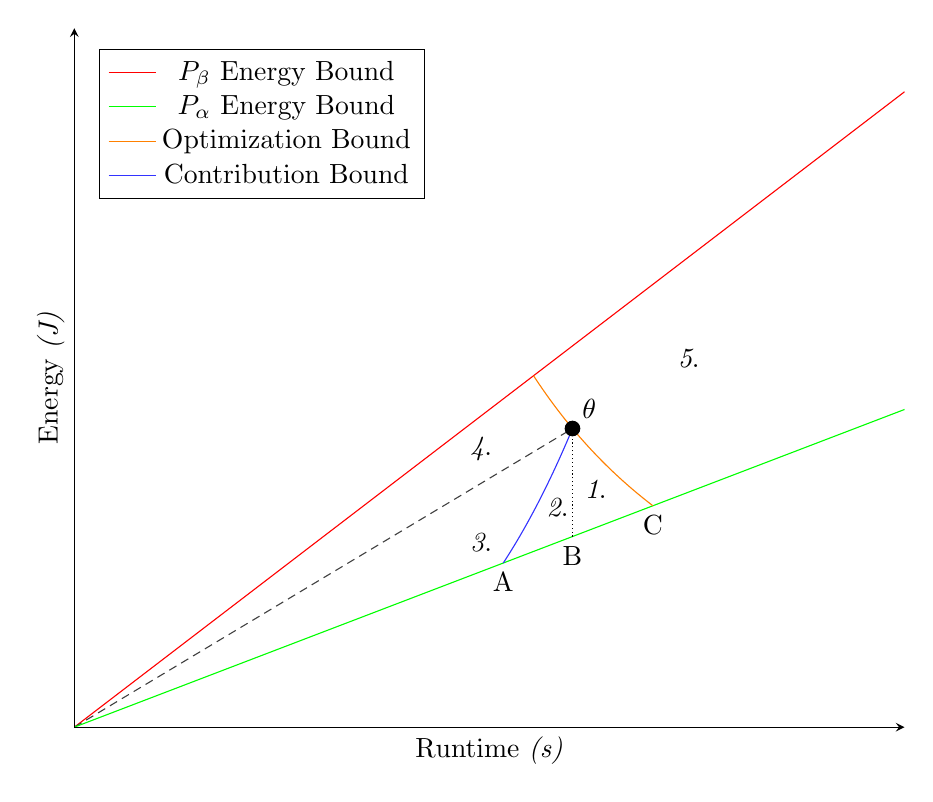
\begin{tikzpicture}
  \begin{axis}[ticks = none, 
    axis on top,
    axis x line=bottom,
    axis y line=left,
  	xlabel={Runtime \emph{(s)}},
    ylabel={Energy \emph{(J)}},    
    xmin=0, xmax=50,
    ymin=0, ymax=3300,
    width=\linewidth,
    legend style={legend pos=north west}
    ]

    %% Model Parameters %%
    \pgfmathsetmacro{\baselinepower}{30} % NOP code
    \pgfmathsetmacro{\rooflinepower}{60}
    \pgfmathsetmacro{\codepower}{47} 
    \pgfmathsetmacro{\codetime}{30}
    % Sadly, pgfplots sucks too much to calculate cube roots
    % These values are calculated with a ruby script in tools
    \pgfmathsetmacro{\anodex}{25.83028}
    \pgfmathsetmacro{\cnodex}{34.84283}
    \pgfmathsetmacro{\tnodex}{27.65477}

    \pgfmathsetmacro{\cnodey}{\cnodex * \baselinepower}
    \pgfmathsetmacro{\anodey}{\anodex * \baselinepower}
 
    %% Intermezzo Values %%
    \pgfmathsetmacro{\codeenergy}{\codepower * \codetime}
    \pgfmathsetmacro{\baselineenergy}{\baselinepower * \codetime}
    \pgfmathsetmacro{\rooflineenergy}{\rooflinepower * \codetime}
    \pgfmathsetmacro{\lowdisplayline}{(2 * \baselinepower + \codepower) / 3}
    \pgfmathsetmacro{\highdisplayline}{(1 * \rooflinepower + 1 * \codepower) / 2}

    % arguments: code power, code time, x - todo, apparently not supposed to do pgfmathparse
    \pgfmathdeclarefunction{metricbound}{3}{%
      \pgfmathparse{((#1 * #2^3) / #3^2)}%
    }
    \pgfmathdeclarefunction{definitionbound}{3}{%
      \pgfmathparse{((#1 / #2^3) * #3^4)}%
    }

    % BETA ROOFLINE BOUND
    \addplot[color=red, domain=\pgfkeysvalueof{/pgfplots/xmin}:\pgfkeysvalueof{/pgfplots/xmax}] {\rooflinepower * x};
    \addlegendentry{$P_{\beta}$ Energy Bound}

    %const power diagonal
    \addplot[color=darkgray, densely dashed, forget plot, %forget plot prevents legend entry
            domain=\pgfkeysvalueof{/pgfplots/xmin}:\codetime] {\codepower * x}; 

    % ALPHA BASELINE BOUND 
    \addplot[color=green, domain=\pgfkeysvalueof{/pgfplots/xmin}:\pgfkeysvalueof{/pgfplots/xmax}] {\baselinepower * x};
    \addlegendentry{$P_{\alpha}$ Energy Bound} 

    \addplot[color=orange, domain=\tnodex:\cnodex] { metricbound(\codepower, \codetime, x)};
    \addlegendentry{Optimization Bound}

    \addplot[color=blue!80, domain=\anodex:\codetime] { definitionbound(\codepower, \codetime, x)};
    \addlegendentry{Contribution Bound}

    % Constant Time, Energy Dashes
    %vertical
    \draw[densely dotted] ({axis cs:\codetime,\baselineenergy}) -- ({axis cs:\codetime,\codeenergy});

    \node[circle,fill,inner sep=2pt] at (axis cs:\codetime,\codeenergy) {};
    \node[above right] at (axis cs:\codetime,\codeenergy) {$\theta$};
    \pgfmathsetmacro{\oneycoord}{\lowdisplayline * 31.4}
    \node at (axis cs:31.4,\oneycoord) {\textit1.};
    \pgfmathsetmacro{\twoycoord}{\lowdisplayline * 29.1}
    \node at (axis cs:29.1,\twoycoord) {\textit2.};
    \pgfmathsetmacro{\threeycoord}{\lowdisplayline * 24.5}
    \node at (axis cs:24.5,\threeycoord) {\textit3.};
    \pgfmathsetmacro{\fourycoord}{\highdisplayline * 24.5}
    \node at (axis cs:24.5,\fourycoord) {\textit4.};
    \pgfmathsetmacro{\fiveycoord}{\codepower * 37}
    \node at (axis cs:37,\fiveycoord) {\textit5.};
    
    \node [below] at ({axis cs:\anodex, \anodey}) {A};
    \node [below] at ({axis cs:\codetime,\baselineenergy}) {B};
    \node [below] at ({axis cs:\cnodex, \cnodey}) {C};
    %\node [below, name intersections={of=metric bound and baseline}] at (intersection-1) {C};


 \end{axis}
\end{tikzpicture}

    \caption{$Et^2$ Power Optimised Software Envelope}
    \label{fig:technique}
    \end{figure}
  \end{frame}
  \begin{frame}
    \frametitle{Feasible Performance Envelope}
  \end{frame}
  \begin{frame}
    \frametitle{Optimisation Bound}
  \end{frame}
  \begin{frame}
    \frametitle{Contribution Bound}
  \end{frame}
  \begin{frame}
    \frametitle{Contribution Limit}
  \end{frame}
  \begin{frame}
    \frametitle{Investigation}
  \end{frame}

%Fragile frames can't be indented. which sucks.
\begin{frame}[fragile]
\frametitle{Baseline Measurement}
\centering                                                                      
\lstset{basicstyle=\ttfamily\footnotesize\bfseries, frame=tb} %small bold text, lines top and bottom 
\lstinputlisting[caption=Baseline Power Microbenchmark]{lst/alpha_benchmark.c}              
\label{fig:microbench}                                                           
\end{frame}

  \begin{frame}
    \frametitle{Roofline Measurement}
      TODO - prime95
  \end{frame}

  \begin{frame}
    \frametitle{Conclusions}
  \end{frame}
  \begin{frame}
    \frametitle{Questions}
  \end{frame}
\end{document}
